\documentclass{article}
\usepackage{lipsum}
\usepackage{booktabs}
\usepackage{graphicx}

\usepackage{amsmath,amsthm,amsfonts}
\usepackage{csquotes}
\newtheorem{theorem}{Theorem}

\theoremstyle{definition}
\newtheorem{definition}{Definition}


\begin{document}
	\title{\LaTeX\ CSS}
	\author{John Doe}
	
	\maketitle
	
	\begin{abstract}
		\lipsum[66]
	\end{abstract}

	\tableofcontents
	
	\section{First Section}
	\lipsum[66]
	 $$(x+y)^{n}=\sum_{k=0}^{n}\left(\begin{array}{l}n \\
		k\end{array}\right) x^{n-k}
	y^{k}=\sum_{k=0}^{n}\left(\begin{array}{l}n \\ k\end{array}\right)
	x^{k} y^{n-k}$$
	\lipsum[75]
	
	\section{Environments}
	\lipsum[75]
	\subsection{Theorem and Proofs}
	\begin{theorem}
		The real numbers $\mathbb{R}$ are uncountable.
	\end{theorem}
	\begin{proof}
	If $\mathbb{R}$ is countable, then [0, 1] is countable as well. Hence
	there exists a map C from $\mathbb{N}$ onto [0, 1] with
	$$C(n)=\sum_{i=1}^{\infty} c_{i}(n) 10^{-i}$$ where $c_{i}(n)
	\in\{0,1, \ldots, 9\},$ are the digits in decimal expansion. Now
	consider a real number $$x=\sum_{i=1}^{\infty} \bar{c}_{i} 10^{-i}
	\in[0,1]$$ with $\bar{c}_{i} \neq c_{i}(i)$. Obviously $C(n) \neq x$
	for all $n \in \mathbb{N} .$ Hence $C$ is not onto. A contradiction.
	\end{proof}

\subsection{Definitions, lemmas...}

\begin{definition}
A definition is a a statement of the meaning of a word or word group or a sign or symbol.
\end{definition}

\section{Formatting Texts}

Some text can be \textbf{bold} and some can be \emph{emphasized.}

\begin{quote}
	Give me six hours to chop down a tree and I will spend the first four sharpening the axe.  \emph{-- Abraham Lincoln}
\end{quote}

\section{Tables and Images}
\lipsum[12]

\begin{table}[h]
	\centering
	\caption{Caption of the table}
	\begin{tabular}{lll}
		\toprule 
	\textbf{Header 1} &\textbf{ Header 2} & \textbf{Header 3} \\
		\toprule
		Text 1 & Text 2 & Text 3 \\ 
		Text 1 & Text 2 & Text 3 \\ 
		Text 1 & Text 2 & Text 3 \\ \bottomrule
		
	\end{tabular}
\end{table}
\lipsum[75]

\begin{figure}[h]
	\centering
	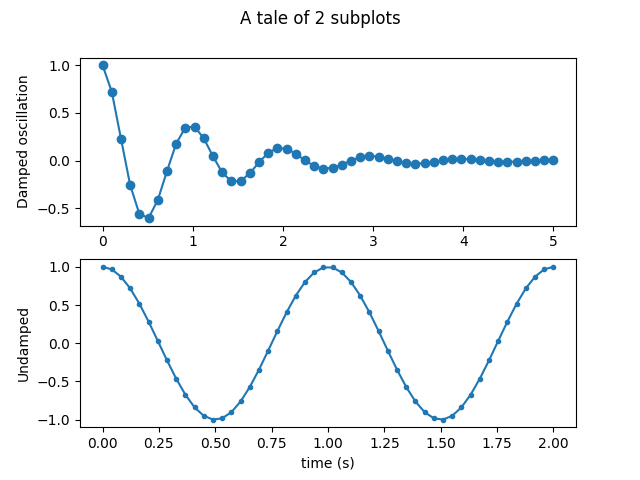
\includegraphics[scale=.5]{img/image}
	\caption{Figure caption}
	
\end{figure}

\section{Syntax Highlighting}

\begin{verbatim}
	\section{Some section...}
	\begin{enumerate}
		\item first element
		\item second element
		\item third element
	\end{enumerate}
\end{verbatim}


	
\end{document}